\documentclass{article}

\usepackage{graphicx}
\usepackage[margin=0.5in]{geometry}
\usepackage{amsmath}
\usepackage{amssymb}
\usepackage[T1]{fontenc}
\usepackage{listings}
\usepackage{psfrag}
\usepackage{alltt}
\usepackage{rotating}


\pagenumbering{gobble}


\begin{document}

\begin{sidewaysfigure}[h!]
	\begin{center}
		\begin{minipage}[h!]{0.8\textwidth}
			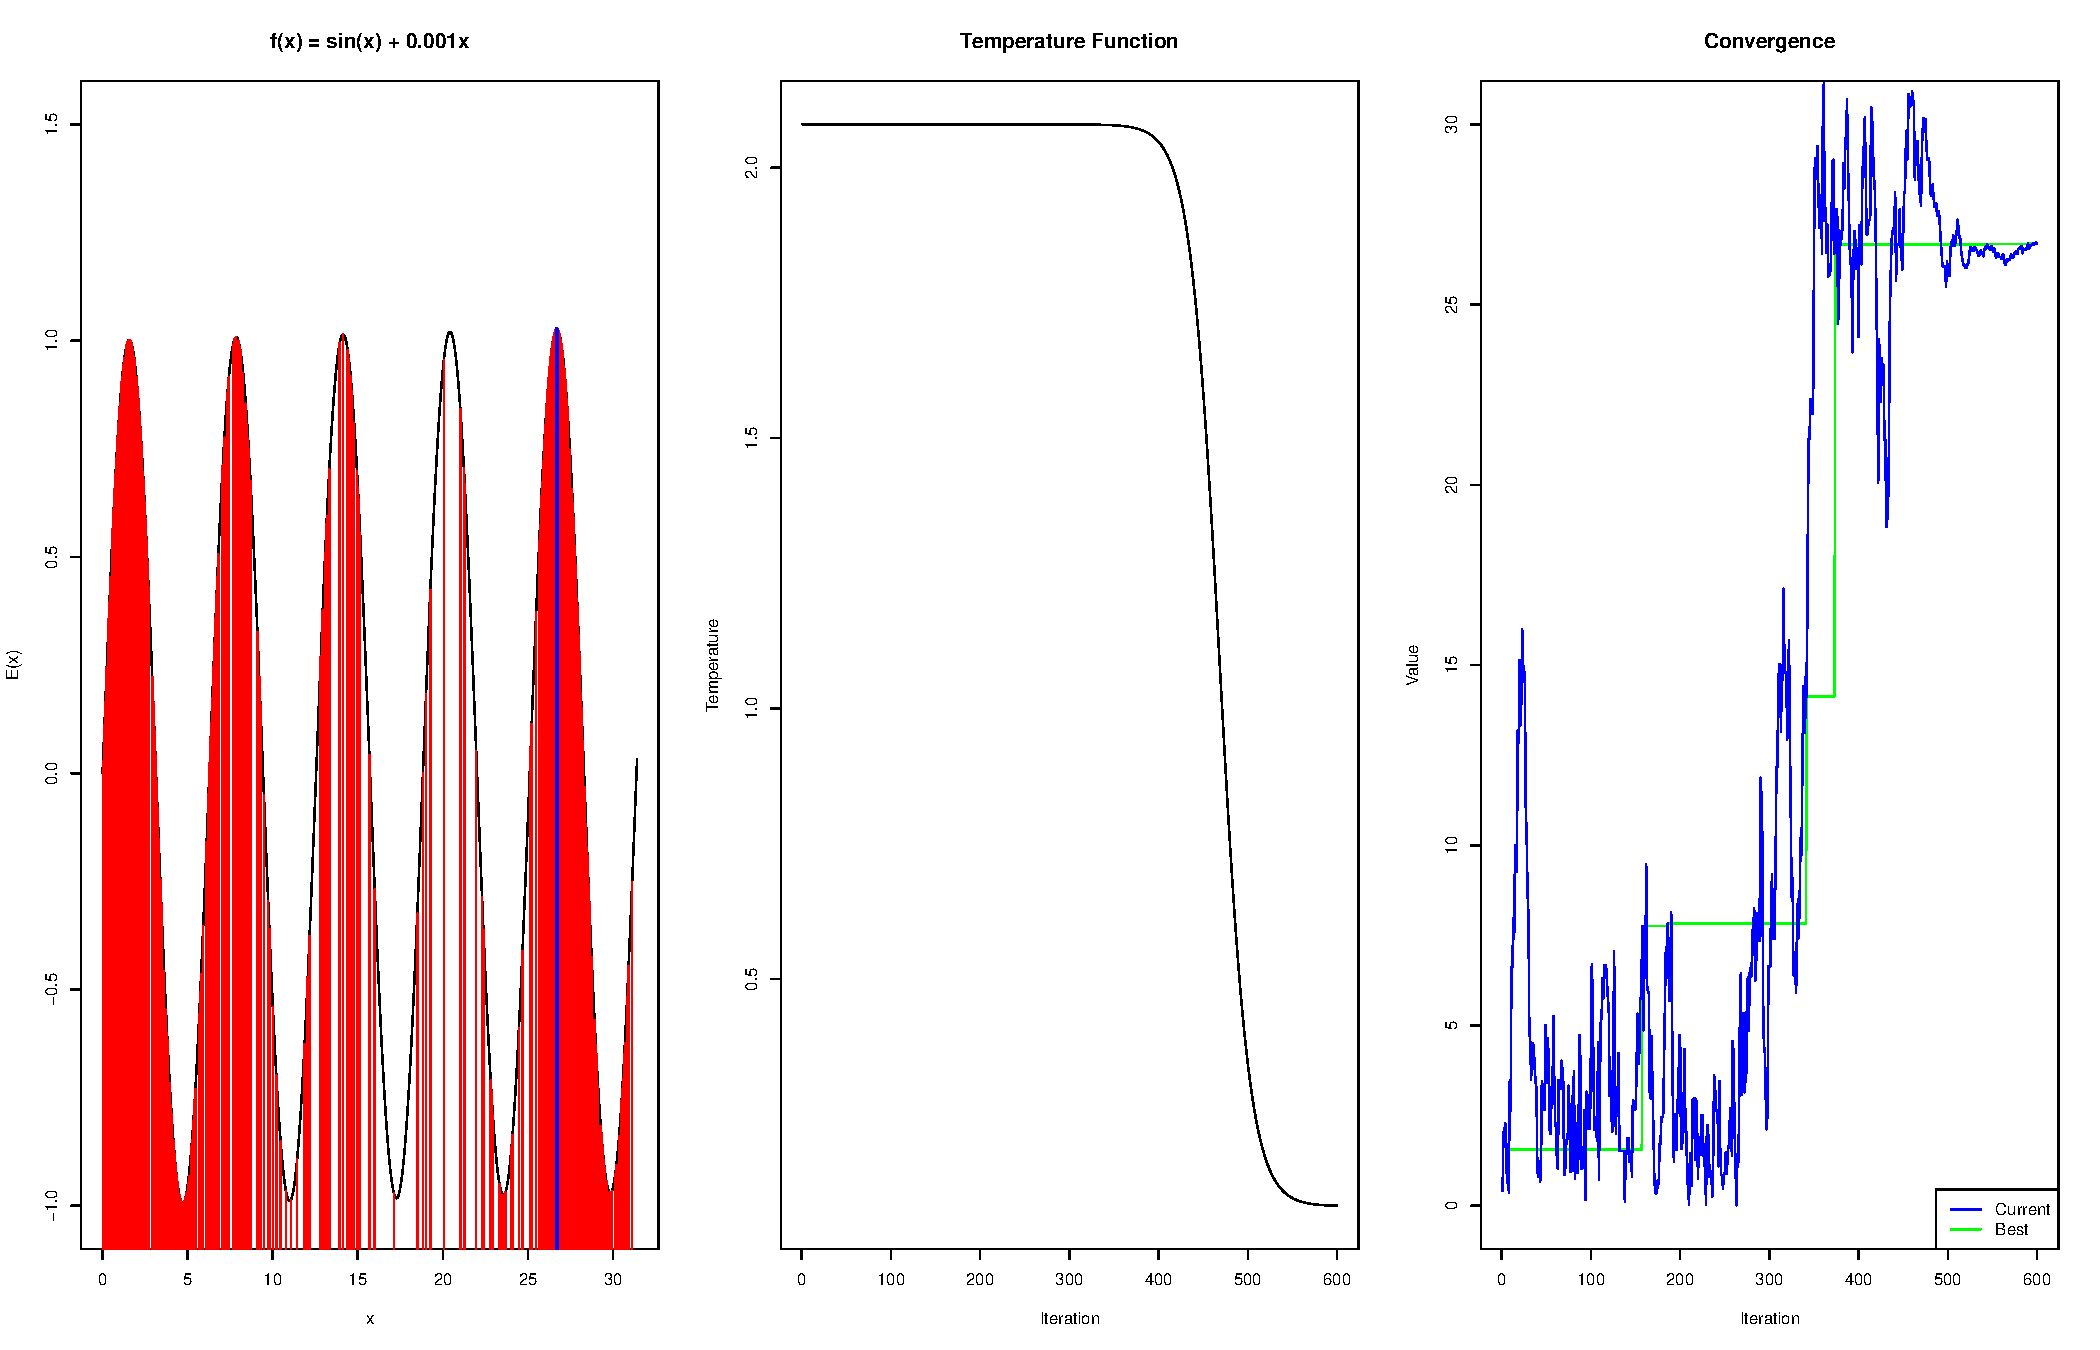
\includegraphics[width=1.0\textwidth]{simPic1.pdf}
		\end{minipage}
		\begin{minipage}[h!]{0.19\textwidth}
			\begin{alltt}
			My Outputs:
			Guess           = 0.000000
			Par             = 26.693205
			Value           = 1.026640
			Iterations      = 600
			Acceptance Rate = 0.861667	
			\end{alltt}
		\end{minipage}
	\end{center}
\end{sidewaysfigure}

\clearpage

\begin{sidewaysfigure}[h!]
	\begin{center}
		\begin{minipage}[h!]{0.49\textwidth}
			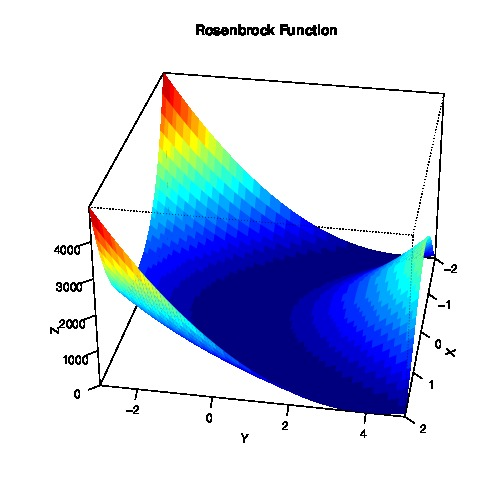
\includegraphics[width=1.0\textwidth]{rosePersp.jpg}
		\end{minipage}
		\begin{minipage}[h!]{0.49\textwidth}
			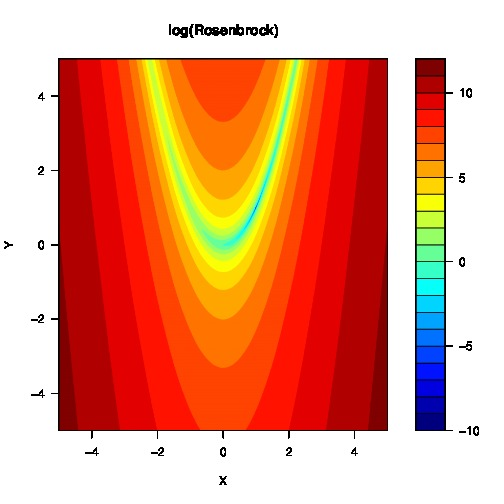
\includegraphics[width=1.0\textwidth]{roseContour.jpg}	
		\end{minipage}
	\end{center}
\end{sidewaysfigure}

\clearpage

\begin{sidewaysfigure}[h!]
	\begin{center}
		\begin{minipage}[h!]{0.66\textwidth}
			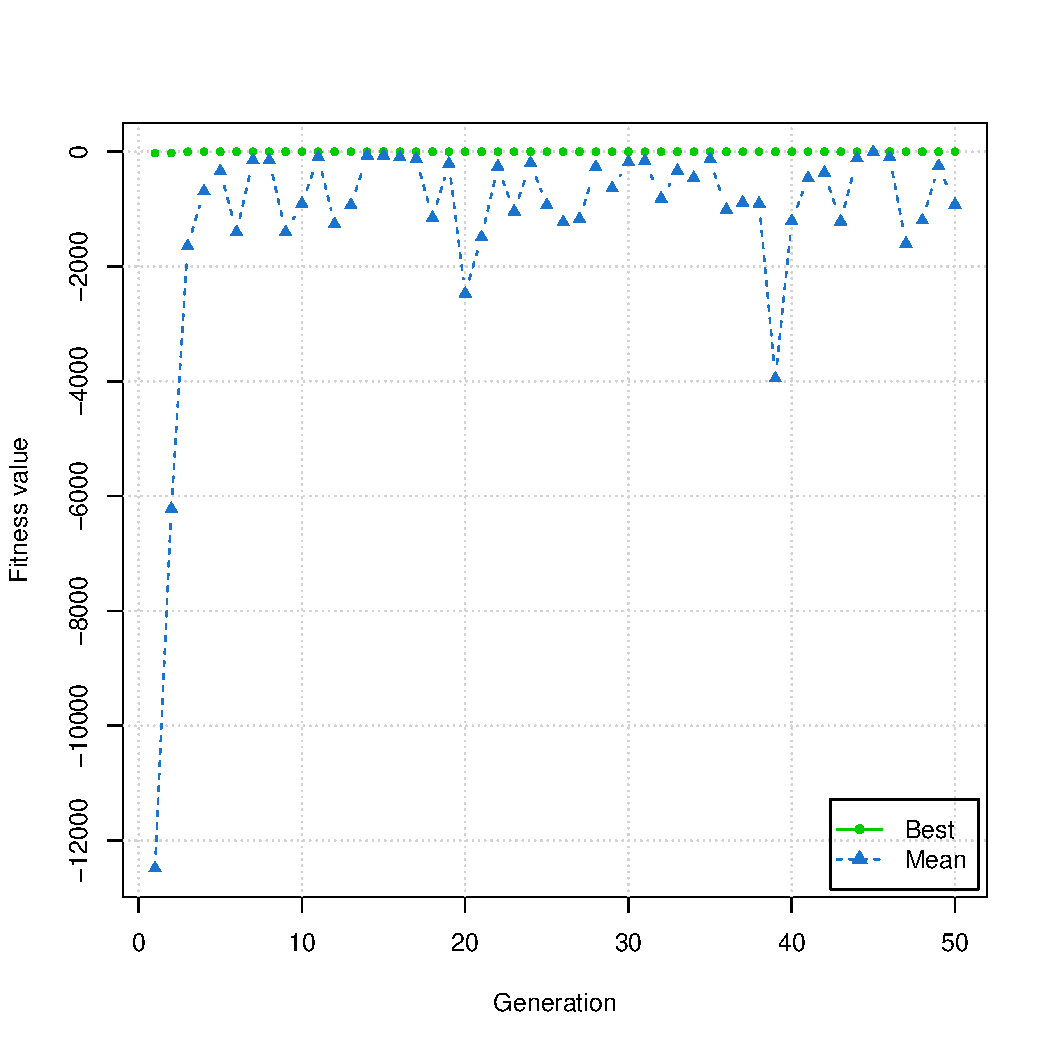
\includegraphics[width=1.0\textwidth]{gaConverge3D.pdf}
		\end{minipage}
		\begin{minipage}[h!]{0.33\textwidth}
			\begin{alltt}
			+-----------------------------------+
			|         Genetic Algorithm         |
			+-----------------------------------+
			
			GA settings: 
			Type                  =  real-valued 
			Population size       =  50 
			Number of generations =  50 
			Elitism               =   
			Crossover probability =  0.8 
			Mutation probability  =  0.1 
			Search domain 
			    x1 x2
			Min -5 -5
			Max  5  5
			
			GA results: 
			Iterations             = 50 
			Fitness function value = -0.001595106 
			Solution               = 
			           x1       x2
			[1,] 1.015345 1.027239
			\end{alltt}	
		\end{minipage}
	\end{center}
\end{sidewaysfigure}

\clearpage

\begin{sidewaysfigure}[h!]
	\begin{center}
		\begin{minipage}[h!]{0.49\textwidth}
			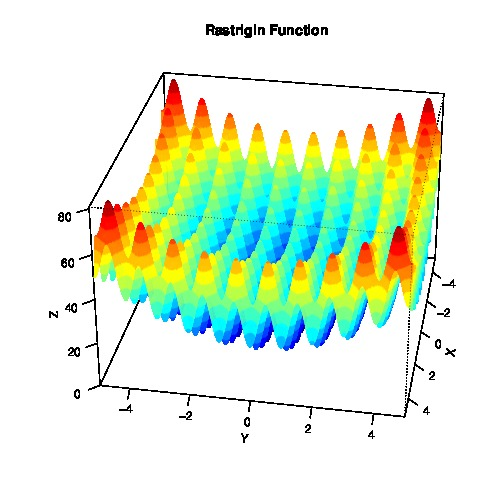
\includegraphics[width=1.0\textwidth]{rastPersp.jpg}
		\end{minipage}
		\begin{minipage}[h!]{0.49\textwidth}
			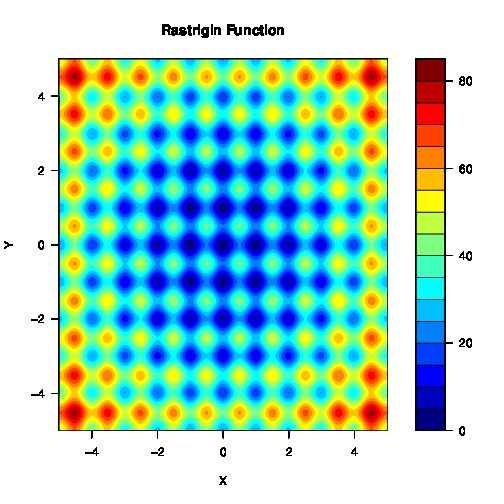
\includegraphics[width=1.0\textwidth]{rastContour.jpg}	
		\end{minipage}
	\end{center}
\end{sidewaysfigure}

\begin{sidewaysfigure}[h!]
	\begin{center}
		\begin{minipage}[h!]{0.66\textwidth}
			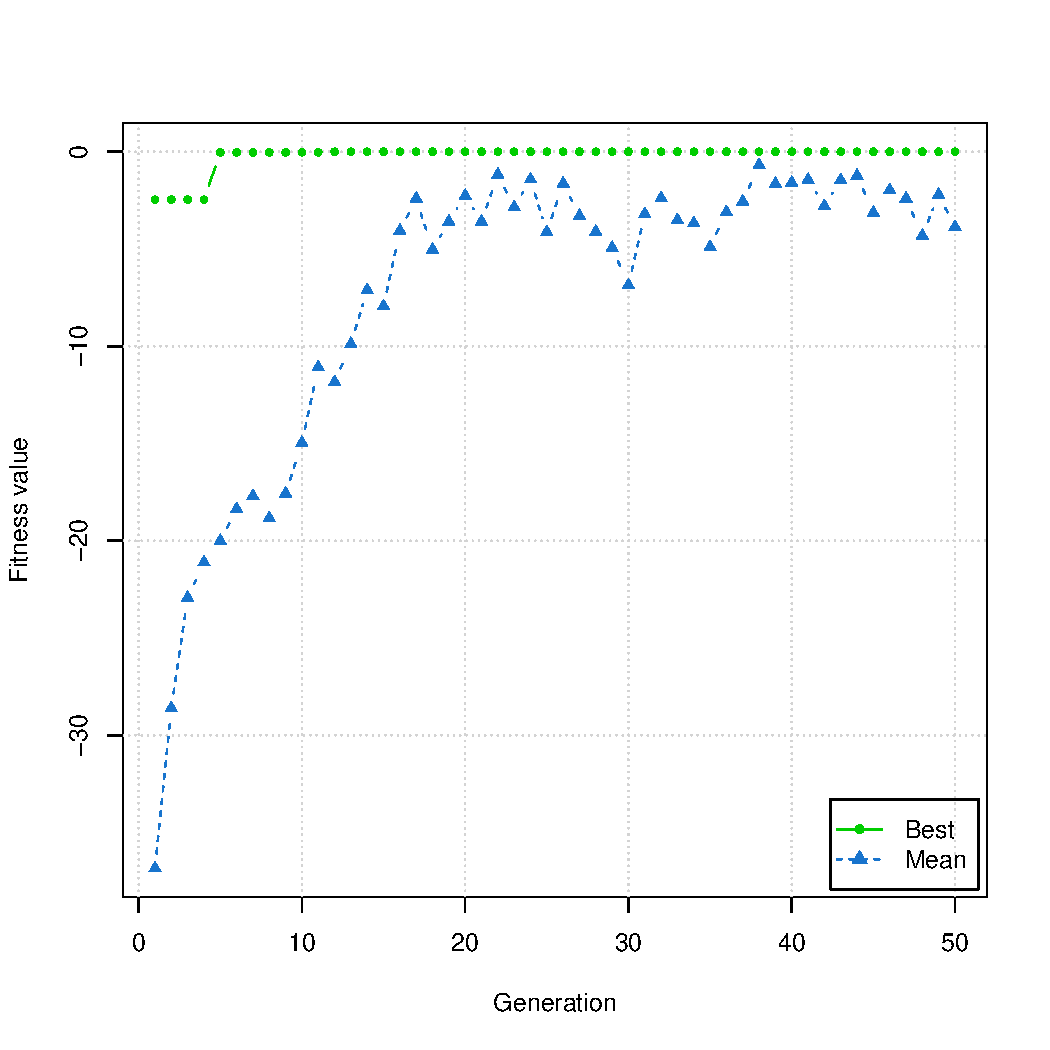
\includegraphics[width=1.0\textwidth]{gaConverge3DRasta.pdf}
		\end{minipage}
		\begin{minipage}[h!]{0.33\textwidth}
			\begin{alltt}
			+-----------------------------------+
			|         Genetic Algorithm         |
			+-----------------------------------+
			
			GA settings: 
			Type                  =  real-valued 
			Population size       =  50 
			Number of generations =  50 
			Elitism               =   
			Crossover probability =  0.8 
			Mutation probability  =  0.1 
			Search domain 
			    x1 x2
			Min -5 -5
			Max  5  5
			
			GA results: 
			Iterations             = 50 
			Fitness function value = -9.598778e-05 
			Solution               = 
			               x1            x2
			[1,] -0.000386534 -0.0005782911
			\end{alltt}	
		\end{minipage}
	\end{center}
\end{sidewaysfigure}

\clearpage

\begin{sidewaysfigure}[h!]
        \begin{center}
                \begin{minipage}[h!]{0.49\textwidth}
                        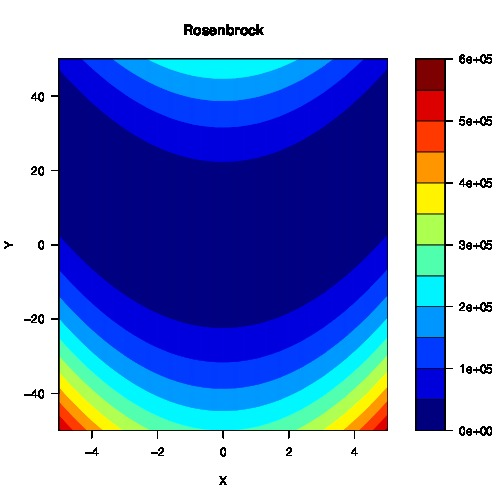
\includegraphics[width=1.0\textwidth]{roseGuesses.jpg}
                \end{minipage}
                \begin{minipage}[h!]{0.49\textwidth}
                        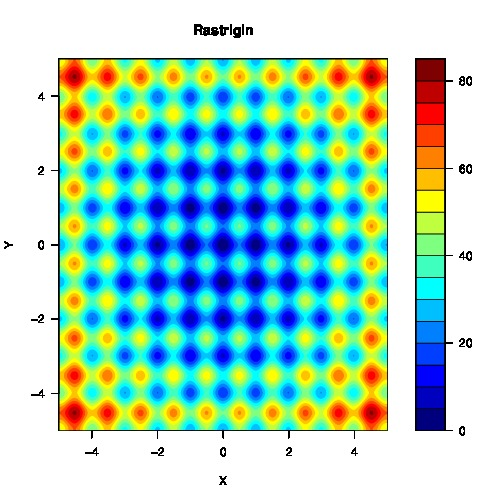
\includegraphics[width=1.0\textwidth]{rastGuesses.jpg}
                \end{minipage}
        \end{center}
\end{sidewaysfigure}

\clearpage

\begin{sidewaysfigure}[h!]
	\begin{center}
		\begin{minipage}[h!]{0.33\textwidth}
			\small\begin{alltt}
			BFGS Rosenbrock Outputs:
			
			Initial Guess: [-4.000, 60.000]
			$par
			[1] 0.9999556 0.9999111
			
			$value
			[1] 1.970508e-09
			
			$counts
			function gradient 
			     303       86 
			
			$convergence
			[1] 0
			
			$message
			NULL
			
			$hessian
			          [,1]      [,2]
			[1,]  801.9298 -399.9822
			[2,] -399.9822  200.0000
			
			
			
			SANN Rosenbrock Outputs:

			Initial Guess: [-4.000, 60.000]
			$par
			[1] -7.572046 57.348046
			
			$value
			[1] 73.49477
			
			$counts
			function gradient 
			   10000       NA 
			
			$convergence
			[1] 0
			
			$message
			NULL
			
			$hessian
			          [,1]     [,2]
			[1,] 45865.843 3028.818
			[2,]  3028.818  200.000	
			\end{alltt}
		\end{minipage}
		\begin{minipage}[h!]{0.33\textwidth}
			\small\begin{alltt}
			BFGS Rosenbrock Outputs:
			
			Initial Guess: [0.000, 0.000]
			$par
			[1] 0.9998000 0.9996001
			
			$value
			[1] 3.998081e-08
			
			$counts
			function gradient 
			      63       26 
			
			$convergence
			[1] 0
			
			$message
			NULL
			
			$hessian
			          [,1]    [,2]
			[1,]  801.6809 -399.92
			[2,] -399.9200  200.00
			
			
			
			SANN Rosenbrock Outputs:
			
			Initial Guess: [0.000, 0.000]
			$par
			[1] 0.9947926 0.9903466
			
			$value
			[1] 8.104591e-05
			
			$counts
			function gradient 
			   10000       NA 
			
			$convergence
			[1] 0
			
			$message
			NULL
			
			$hessian
			          [,1]     [,2]
			[1,]  793.3969 -397.917
			[2,] -397.9170  200.000
			
			\end{alltt}	
		\end{minipage}
		\begin{minipage}[h!]{0.33\textwidth}
			\small\begin{alltt}
			BFGS Rosenbrock Outputs:
			
			Initial Guess: [-5.000, -50.000]
			$par
			[1] 0.9999050 0.9998105
			
			$value
			[1] 9.034556e-09
			
			$counts
			function gradient 
			     171       58 
			
			$convergence
			[1] 0
			
			$message
			NULL
			
			$hessian
			          [,1]     [,2]
			[1,]  801.8487 -399.962
			[2,] -399.9620  200.000
			
			

			SANN Rosenbrock Outputs:

			Initial Guess: [-5.000, -50.000]
			$par
			[1] 0.9952577 0.9916683
			
			$value
			[1] 0.0001502636
			
			$counts
			function gradient 
			   10000       NA 
			
			$convergence
			[1] 0
			
			$message
			NULL
			
			$hessian
			          [,1]      [,2]
			[1,]  793.9790 -398.1031
			[2,] -398.1031  200.0000			
			\end{alltt}
		\end{minipage}
	\end{center}
\end{sidewaysfigure}

\clearpage

\begin{sidewaysfigure}[h!]
	\begin{center}
		\begin{minipage}[h!]{0.33\textwidth}
			\small\begin{alltt}
			BFGS Rastigin Outputs:

			Initial Guess: [-5.000, 5.000]
			$par
			[1] -5.094763e-10  5.094763e-10
			
			$value
			[1] 0
			
			$counts
			function gradient 
			      29        3 
			
			$convergence
			[1] 0
			
			$message
			NULL
			
			$hessian
			        [,1]    [,2]
			[1,] 396.779   0.000
			[2,]   0.000 396.779
			
			

			SANN Rastigin Outputs:
			
			Initial Guess: [-5.000, 5.000]
			$par
			[1] 0.001099102 3.980160587
			
			$value
			[1] 15.91951
			
			$counts
			function gradient 
			   10000       NA 
			
			$convergence
			[1] 0
			
			$message
			NULL
			
			$hessian
			         [,1]     [,2]
			[1,] 396.7696   0.0000
			[2,]   0.0000 393.7158						
			\end{alltt}
		\end{minipage}
		\begin{minipage}[h!]{0.33\textwidth}
			\small\begin{alltt}
			BFGS Rastigin Outputs:
			
			Initial Guess: [1.000, -1.000]
			$par
			[1]  0.9949586 -0.9949586
			
			$value
			[1] 1.989918
			
			$counts
			function gradient 
			      19        3 
			
			$convergence
			[1] 0
			
			$message
			NULL
			
			$hessian
			             [,1]         [,2]
			[1,] 3.965809e+02 8.881784e-10
			[2,] 8.881784e-10 3.965809e+02
			
			
			
			SANN Rastigin Outputs:
			
			Initial Guess: [1.000, -1.000]
			$par
			[1] -0.9945749  0.9939758
			
			$value
			[1] 1.990139
			
			$counts
			function gradient 
			   10000       NA 
			
			$convergence
			[1] 0
			
			$message
			NULL
			
			$hessian
			         [,1]     [,2]
			[1,] 396.5497   0.0000
			[2,]   0.0000 396.4962	
			\end{alltt}	
		\end{minipage}
		\begin{minipage}[h!]{0.33\textwidth}
			\small\begin{alltt}
			BFGS Rastigin Outputs:
			
			Initial Guess: [1.000, 0.000]
			$par
			[1] 0.9949586 0.0000000
			
			$value
			[1] 0.9949591
			
			$counts
			function gradient 
			      19        3 
			
			$convergence
			[1] 0
			
			$message
			NULL
			
			$hessian
			         [,1]    [,2]
			[1,] 396.5809   0.000
			[2,]   0.0000 396.779
			
			
			
			SANN Rastigin Outputs:
			
			Initial Guess: [1.000, 0.000]
			$par
			[1] 1 0
			
			$value
			[1] 1
			
			$counts
			function gradient 
			   10000       NA 
			
			$convergence
			[1] 0
			
			$message
			NULL
			
			$hessian
			        [,1]    [,2]
			[1,] 396.779   0.000
			[2,]   0.000 396.779			
			\end{alltt}
		\end{minipage}
	\end{center}
\end{sidewaysfigure}









































%
%\begin{sidewaysfigure}[h!]
%\centering
%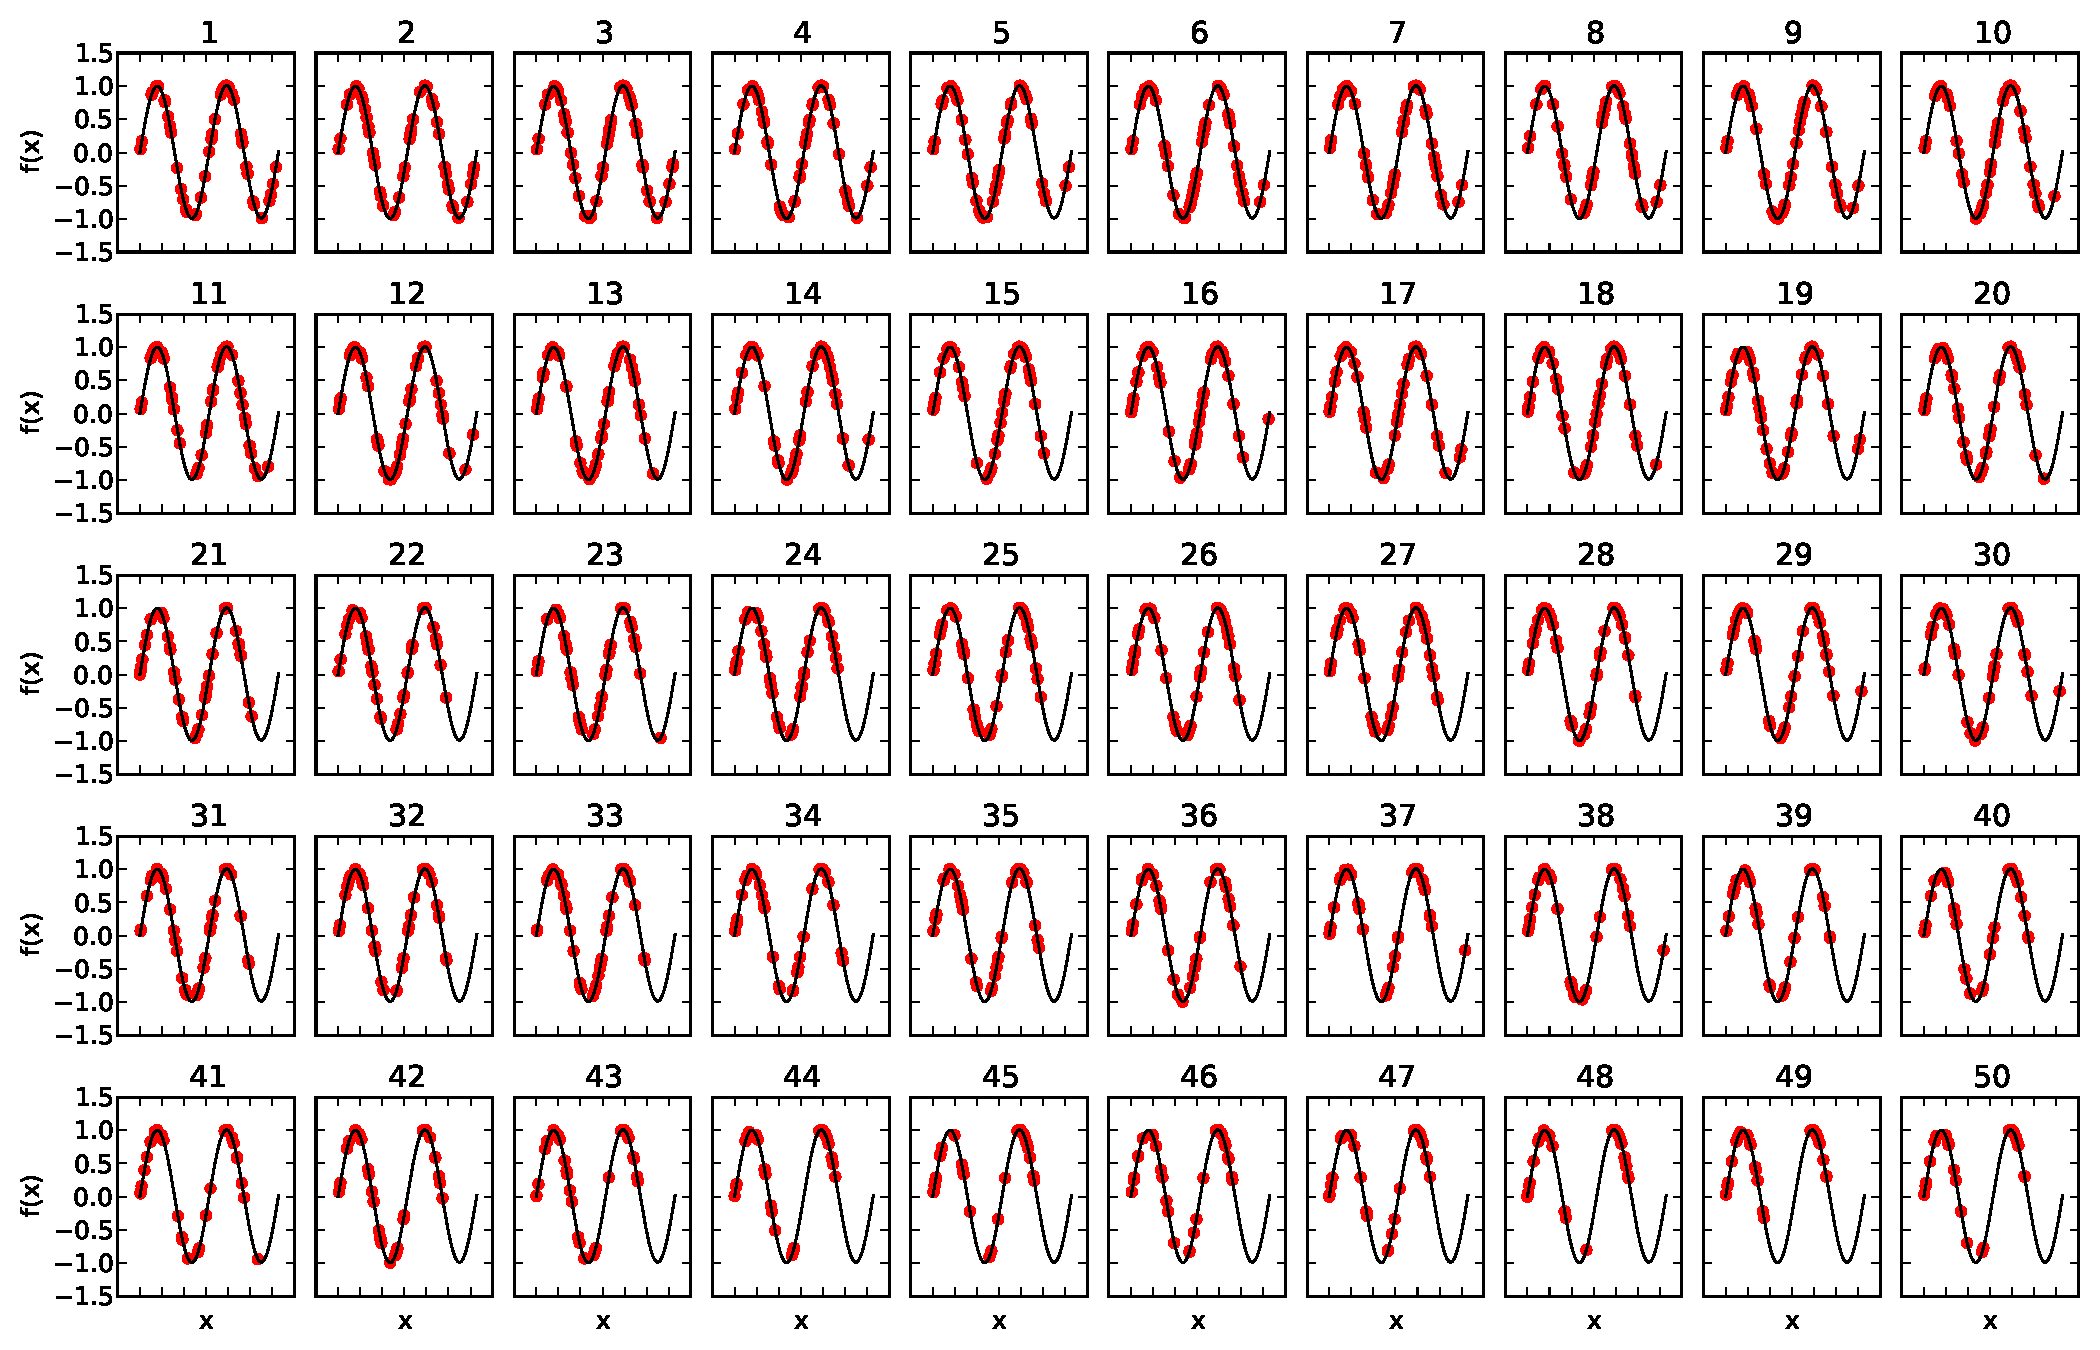
\includegraphics[width=1.0\textwidth]{gaSearchingMe.pdf}
%\end{sidewaysfigure}
%
%\clearpage
%
%\begin{sidewaysfigure}[h!]
%        \begin{center}
%                \begin{minipage}[h!]{0.7\textwidth}
%                        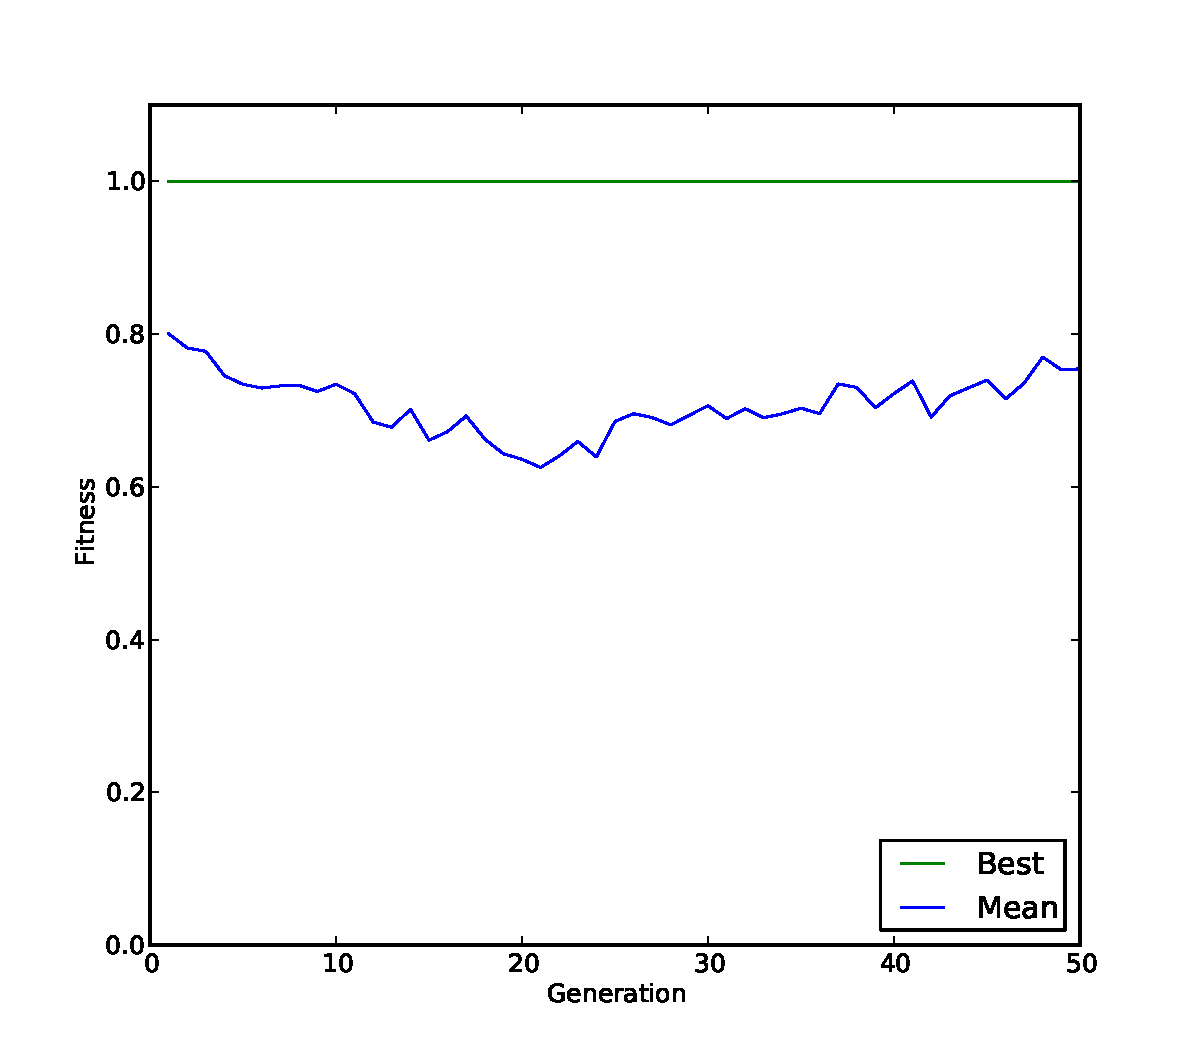
\includegraphics[width=\textwidth]{gaConvergeMe.pdf}
%                \end{minipage}
%                \begin{minipage}[h!]{0.29\textwidth}
%                        \begin{alltt}
%			      My Genetic Algorithm
%			________________________________
%			
%			Population Size       = 50
%			Number of Generations = 50
%			Crossover Probability = 0.20
%			Search Domain: [0.00, 12.57]
%			Precision             = 2
%			
%			            Results  
%			________________________________
%			
%			Fitness               = 1.007842
%			argmax                = 7.86
%                        \end{alltt}
%                \end{minipage}
%        \end{center}
%\end{sidewaysfigure}
%
%\clearpage
%
%
%\begin{sidewaysfigure}[h!]
%	\begin{center}
%		\begin{minipage}[h!]{0.2\textwidth}
%			\begin{alltt}
%				My Outputs:
%				Guess      = 2.000000
%				Par        = 1.571796
%				Value      = 1.001571
%				Iterations = 50
%				Hessian    = -1.000089			
%			\end{alltt}
%		\end{minipage}
%		\begin{minipage}[h!]{0.19\textwidth}
%			\begin{alltt}
%				Optim Outputs:
%				$par
%				[1] 1001133
%				
%				$value
%				[1] 1002.133
%				
%				$counts
%				function gradient 
%				       2        1 
%				
%				$convergence
%				[1] 0
%				
%				$message
%				NULL
%				
%				$hessian
%				           [,1]
%				[1,] -0.9999992
%			\end{alltt}
%		\end{minipage}	
%		\begin{minipage}[h!]{0.6\textwidth}
%			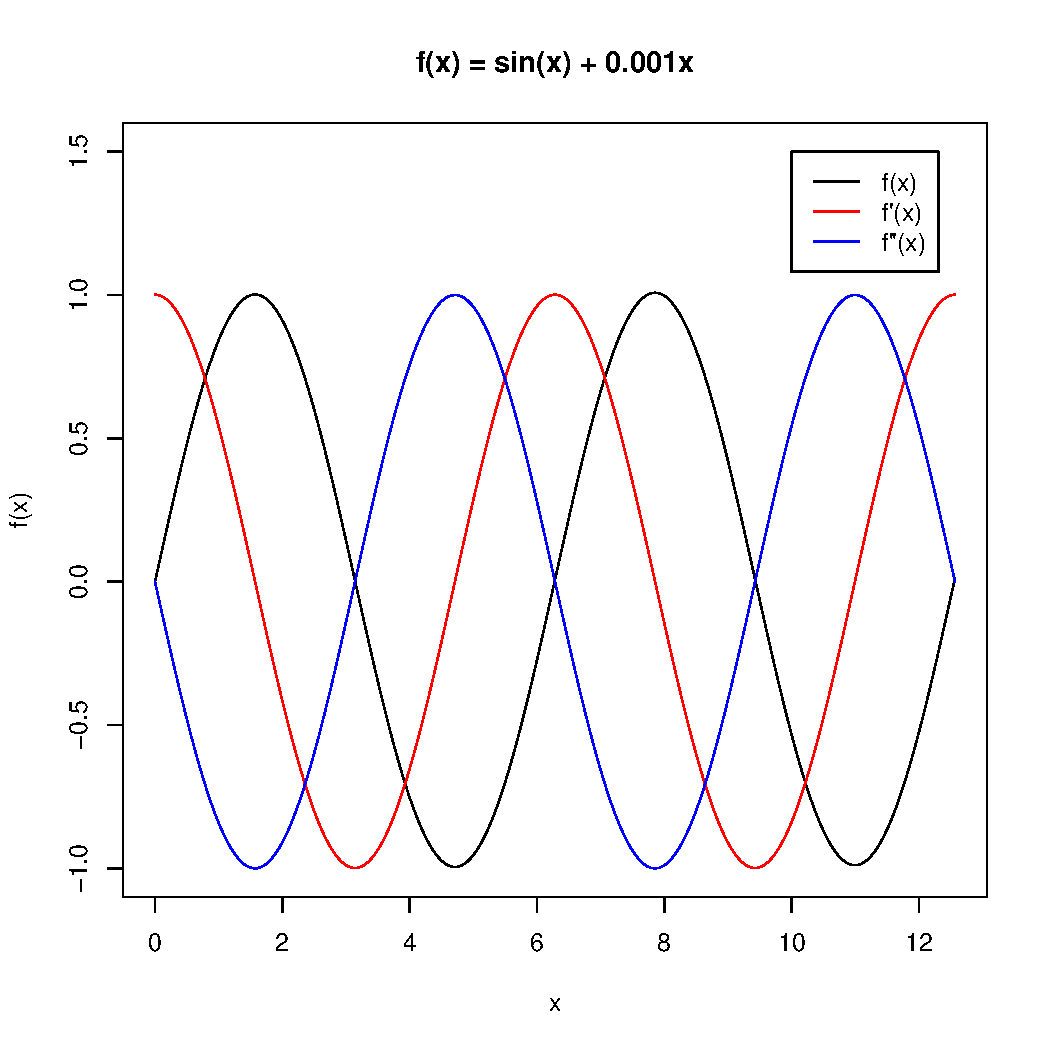
\includegraphics[width=\textwidth]{triggy.pdf}	
%		\end{minipage}			
%	\end{center}
%\end{sidewaysfigure}
%
%\clearpage
%
%\begin{sidewaysfigure}[h!]
%        \begin{center}
%                \begin{minipage}[h!]{0.16\textwidth}
%                        \begin{alltt}
%				My Outputs:
%				Guess      = -2.000000
%				Par        = -0.666667
%				Value      = 0.148148
%				Iterations = 50
%				Hessian    = -2.000011
%          
%                        \end{alltt}
%                \end{minipage}
%                \begin{minipage}[h!]{0.16\textwidth}
%                        \begin{alltt}
%				Optim Outputs:
%				$par
%				[1] -0.6666668
%				
%				$value
%				[1] 0.1481481
%				
%				$counts
%				function gradient 
%				       3        1 
%				
%				$convergence
%				[1] 0
%				
%				$message
%				NULL
%				
%				$hessian
%				          [,1]
%				[1,] -2.000001
%                        \end{alltt}
%                \end{minipage}
%		\begin{minipage}[h!]{0.16\textwidth}
%                        \begin{alltt}
%					My Outputs:
%				Guess      = 0.000000
%				Par        = -0.000001
%				Value      = 0.000000
%				Iterations = 50
%				Hessian    = 2.000003 
%                        \end{alltt}
%                \end{minipage}
%                \begin{minipage}[h!]{0.16\textwidth}
%                        \begin{alltt}
%				Optim Outputs:
%				$par
%				[1] -5.000001e-07
%				
%				$value
%				[1] 2.5e-13
%				
%				$counts
%				function gradient 
%				       5        1 
%				
%				$convergence
%				[1] 0
%				
%				$message
%				NULL
%				
%				$hessian
%				         [,1]
%				[1,] 1.999997		
%                        \end{alltt}
%                \end{minipage} 
%		 \begin{minipage}[h!]{0.16\textwidth}
%                        \begin{alltt}
%				My Outputs:
%				Guess      = 2.000000
%				Par        = -0.000001
%				Value      = 0.000000
%				Iterations = 50
%				Hessian    = 2.000003
%                        \end{alltt}
%                \end{minipage}
%                \begin{minipage}[h!]{0.16\textwidth}
%                        \begin{alltt}
%				Optim Outputs:
%				$par
%				[1] -5.000001e-07
%				
%				$value
%				[1] 2.5e-13
%				
%				$counts
%				function gradient 
%				       5        1 
%				
%				$convergence
%				[1] 0
%				
%				$message
%				NULL
%				
%				$hessian
%				         [,1]
%				[1,] 1.999997
%                        \end{alltt}
%                \end{minipage}
%        \end{center}
%\end{sidewaysfigure}
%
%\clearpage
%
%\begin{sidewaysfigure}[h!]
%	\begin{center}
%		\begin{minipage}[h!]{0.49\textwidth}
%			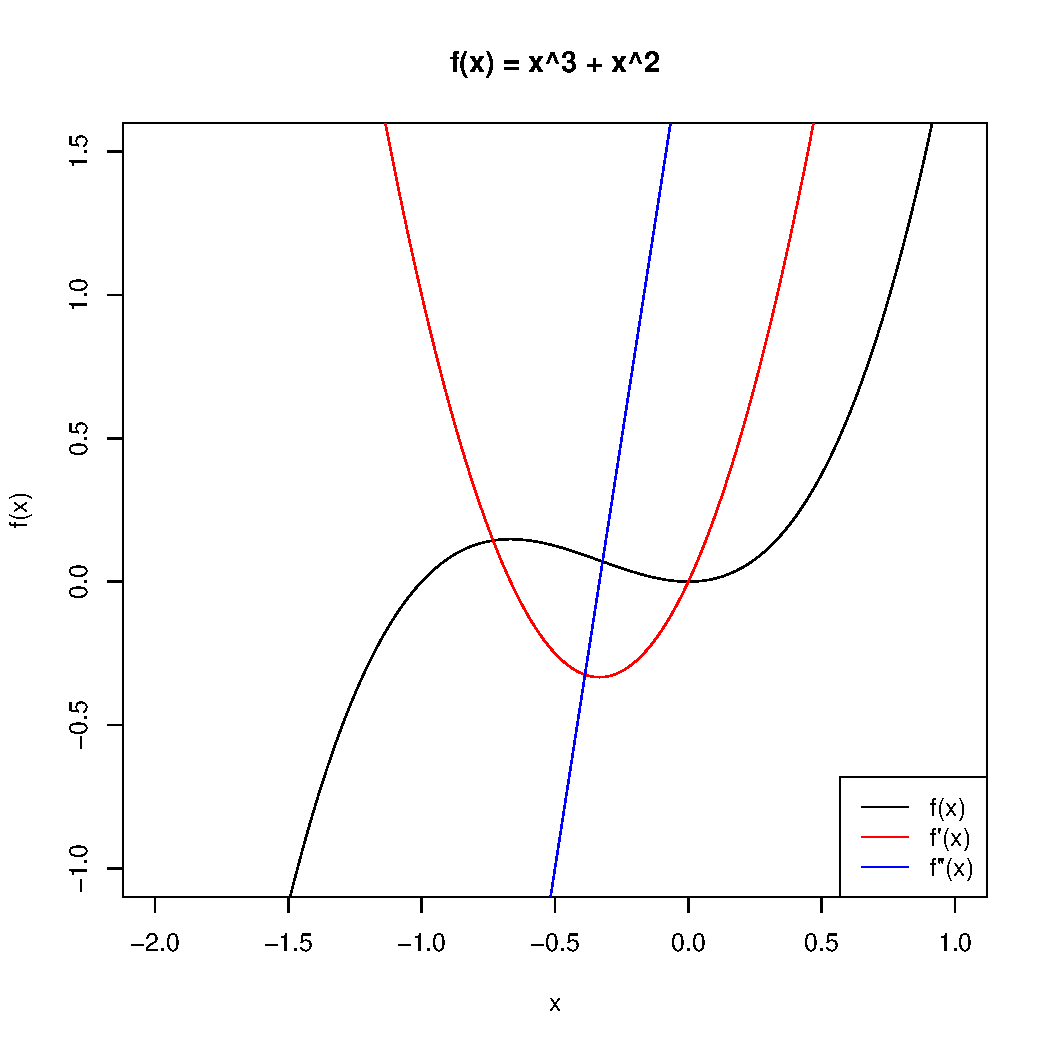
\includegraphics[width=1.0\textwidth]{poly32.pdf}
%		\end{minipage}
%		\begin{minipage}[h!]{0.49\textwidth}
%			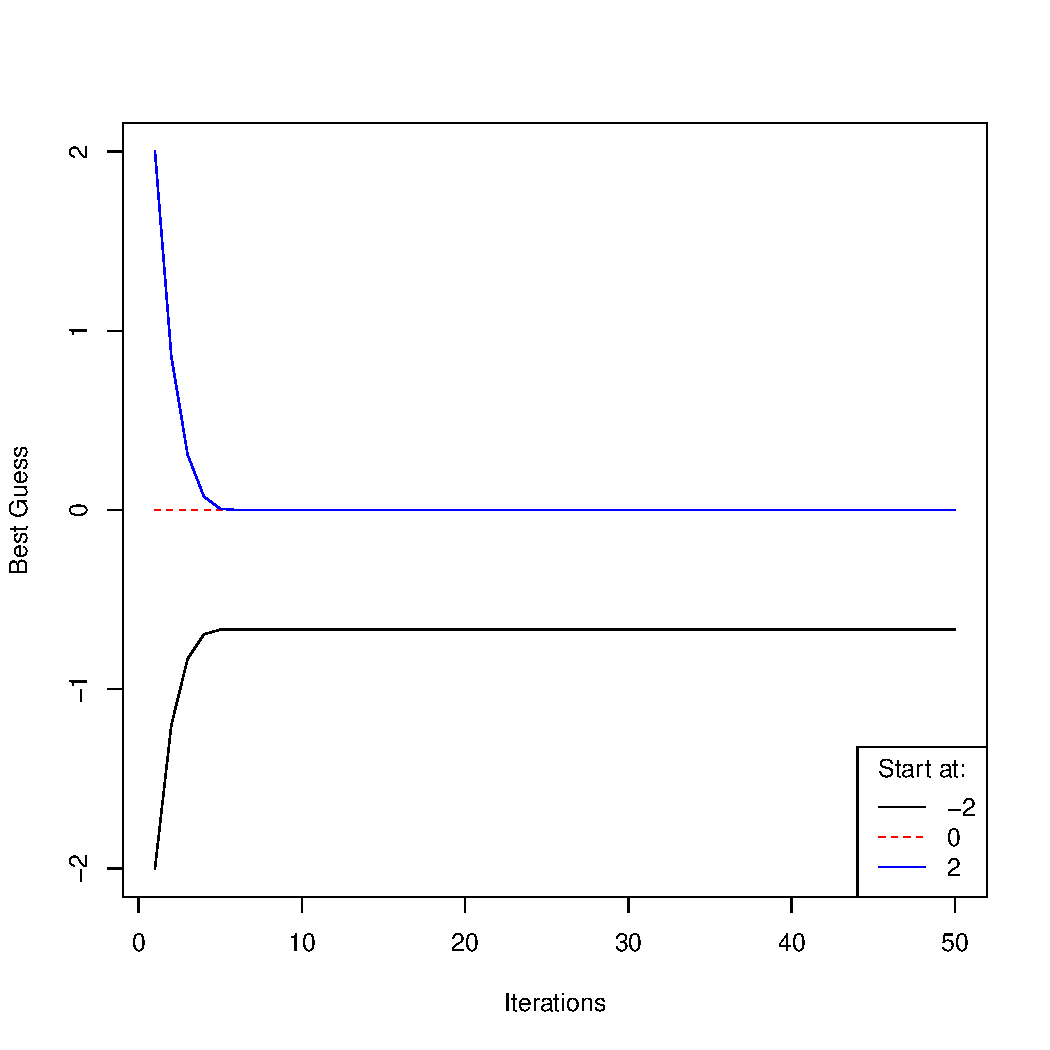
\includegraphics[width=1.0\textwidth]{gradConvergePoly32.pdf}
%		\end{minipage}
%	\end{center}
%\end{sidewaysfigure}
%
%
\end{document}
